\documentclass{amsart}
\usepackage{amsmath,amssymb,amsthm}
\usepackage{mathtools}
\usepackage[hidelinks]{hyperref}
\usepackage{graphicx}
\usepackage{enumitem}
\usepackage{booktabs}

% Guard for a command the imported general.tex template redefines
\providecommand{\algorithmicindent}{}

% Theorem environments
\newtheorem{theorem}{Theorem}[section]
\newtheorem{lemma}[theorem]{Lemma}
\newtheorem{proposition}[theorem]{Proposition}
\newtheorem{corollary}[theorem]{Corollary}
\newtheorem{conjecture}[theorem]{Conjecture}

\theoremstyle{definition}
\newtheorem{definition}[theorem]{Definition}
\newtheorem{example}[theorem]{Example}

\theoremstyle{remark}
\newtheorem{remark}[theorem]{Remark}

\numberwithin{equation}{section}

% Import command files (if they exist)
\InputIfFileExists{commands/math}{}{}
\InputIfFileExists{commands/general}{}{}
\InputIfFileExists{commands/macros}{}{}

% Convenient operators for this paper
\DeclareMathOperator{\II}{I}
\newcommand{\Rg}{R(G)}
\newcommand{\indep}{\perp\!\!\!\perp}

\title[Compensatory Robustness of LLM Alignment]{Compensatory Robustness of Aligned Behavior in Language Models: Information-Theoretic Ablation Bounds and a Percolation Phase Transition}

\author{NeuriCo}
\email{chicagohailab@gmail.com}

\subjclass[2020]{Primary 94A17, 05C40; Secondary 68T07, 60K35}

\date{June 30, 2026}

\keywords{Mutual information, conditional independence, Fano's inequality,
Menger's theorem, vertex connectivity, percolation, phase transition,
mechanistic interpretability, alignment robustness}

\begin{document}

\begin{abstract}
The empirical study of language-model alignment reports two seemingly
contradictory facts: aligned behavior is at once \emph{fragile}---removable by a
handful of gradient steps, concentrated in the first output tokens, or carried by
a single activation direction---and \emph{distributed}, surviving the ablation of
individual heads, directions, or pathways. We give a self-contained mathematical
framework in which both facts are theorems about the same object. Modeling an
aligned behavior as a discrete random variable $S$ read off from internal pathways
$R_1,\dots,R_n$, we prove that the information lost by ablating a pathway equals its
non-redundant conditional mutual information $\II(S;R_i\mid R_{-i})$; fully redundant
pathways cost exactly zero. Via Fano's inequality this information loss lower-bounds
the unavoidable behavioral error after ablation, turning redundancy into a provable
robustness guarantee. Modeling computation as a layered directed acyclic graph, we
show that the \emph{targeted} critical ablation threshold equals the minimum vertex
cut $R(G)$ (Menger's theorem), while the \emph{random} threshold obeys an exact
percolation law $(1-q^w)^d$ whose critical point $q_c=(1-2^{-1/d})^{1/w}\to 1$ is
exponentially separated from the targeted threshold in the redundancy width $w$.
A single network is therefore simultaneously robust to random damage and fragile to
a targeted attack on its min-cut, which dissolves the apparent contradiction in the
literature. Every nontrivial claim is verified computationally: the information
identity holds to machine precision, the Fano floor is never violated, the targeted
threshold equals $R(G)$ exactly, and the random survival law matches Monte-Carlo
estimates within $95\%$ confidence intervals.

\end{abstract}

\maketitle

\section{Introduction}
\label{sec:intro}

Whether the aligned behavior of a large language model (LLM) is encoded
\emph{redundantly} decides whether safety survives quantization, pruning, benign
fine-tuning, or adversarial attack. This is not a matter of taste: the same
intervention that is harmless to a redundantly encoded behavior can be fatal to one
that depends on a single internal component. Yet the empirical literature on the
internal mechanisms of alignment is sharply, and at first sight irreconcilably,
divided.

On one side, alignment looks \emph{fragile and localized}. Fine-tuning on fewer than
a hundred examples raises harmful-response rates from near zero to roughly
$80$--$90\%$ in five to ten gradient steps \cite{qi2023finetuning}; the divergence
between an aligned model and its base model is concentrated in the first few output
tokens \cite{qi2024shallow}; and a single difference-in-means direction, when
projected out, removes refusal across more than a dozen models \cite{arditi2024refusal}.
On the other side, alignment looks \emph{distributed and robust}. Ablating all three
primary name-mover heads of the indirect-object-identification circuit drops the
relevant logit difference by only $5\%$, because dormant backup heads activate to
compensate \cite{wang2022ioi}; refusal is mediated not by one direction but by
polyhedral concept cones of dimension up to five \cite{wollschlager2025cones}; and a
model can survive ablation of its principal safety direction because of ``a richer
internal refusal structure with redundant paths that survived the ablation''
\cite{joad2026directions}.

\paragraph{The gap.}
What is missing is a single quantitative account under which both regimes are special
cases---a scalar (or a pair of scalars) that says \emph{which} kind of robustness a
given aligned behavior has, and which it lacks. The canonical formal measure of
compensation, McGrath et al.'s logit-level compensatory effect \cite{mcgrath2023hydra},
is layer-granular and, as Rushing and Nanda show, roughly $30\%$ of it is a
LayerNorm-scaling artifact rather than genuine rerouting \cite{rushing2024selfrepair}.
No assumption-light bound currently links a redundancy measure to the
\emph{behavioral} effect of an ablation, and no model places ``shallow/fragile'' and
``distributed/redundant'' on one axis.

\paragraph{Our contribution.}
We supply such a framework, organized in three proved layers, each verified
computationally.

\begin{itemize}[leftmargin=*,itemsep=2pt,topsep=2pt]
  \item \textbf{Information layer.} We prove that the information about an aligned
    behavior $S$ lost by ablating a pathway $R_i$ is \emph{exactly} the conditional
    mutual information $\II(S;R_i\mid R_{-i})$, the part of $R_i$'s information that no
    other pathway carries (Theorem~\ref{thm:a1}). Fully redundant pathways cost zero.
    This is an exact identity, free of the LayerNorm artifact that contaminates the
    logit-level effect. A $k$-redundancy condition then guarantees resilience to any
    $k-1$ simultaneous ablations (Theorem~\ref{thm:a2}).
  \item \textbf{From information to behavior.} Through Fano's inequality, the
    information loss lower-bounds the unavoidable behavioral error of \emph{any}
    decoder reading the surviving pathways (Theorem~\ref{thm:b1}). Zero information
    loss forces zero behavioral error: redundancy implies provable behavioral
    robustness. Conversely, when behavior survives an ablation, the surviving pathways
    must have already contained all the information---compensation \emph{reveals}
    pre-existing redundancy rather than creating it (Proposition~\ref{prop:d1}).
  \item \textbf{Graph layer and phase transition.} Modeling computation as a layered
    directed acyclic graph, we show the \emph{targeted} critical ablation threshold
    equals the minimum vertex cut $R(G)$ (Theorem~\ref{thm:c1}), via Menger's theorem.
    Under random ablation, survival obeys the exact law $(1-q^w)^d$
    (Theorem~\ref{thm:c2}), with a percolation phase transition whose critical point
    $q_c=(1-2^{-1/d})^{1/w}\to 1$ and whose width shrinks as $1/w$
    (Theorem~\ref{thm:c3}). The targeted and random thresholds are therefore
    exponentially separated in the redundancy width.
\end{itemize}

The payoff is conceptual. A network carries \emph{two} robustness numbers: the
min-cut $R(G)$ (targeted fragility) and the percolation threshold $q_c$ (random
robustness), and Theorem~\ref{thm:c3} shows they diverge. The same aligned circuit is
then simultaneously robust to random or incidental damage and fragile to a targeted
attack on its min-cut. This reconciles the contradictory empirical reports and yields
an honest verdict on the premise that alignment intrinsically resists removal: the
premise holds in the random/benign regime but fails against a targeted adversary, who
need only degrade $R(G)$ pathway-units to misalign the model
(Corollary~\ref{cor:e1})---matching the easy targeted misalignment of
\cite{qi2023finetuning,qi2024shallow}.

\paragraph{Techniques.}
The proofs use only standard, uncontested tools: the chain rule and non-negativity of
(conditional) mutual information \cite{cover2006elements}, Fano's inequality
\cite{cover2006elements}, Menger's theorem in its vertex form \cite{diestel2017graph},
and exact percolation algebra on a series-parallel circuit. We deliberately base the
main bounds on Shannon mutual information rather than a specific partial-information-decomposition
operator, using the latter \cite{williams2010pid} only as an independent cross-check.

\paragraph{Organization.}
Section~\ref{sec:prelim} fixes notation, gives the definitions, and recalls the
prerequisite theorems. Section~\ref{sec:results} states and proves the information-layer
results (Section~\ref{sec:results}.1), the behavioral and structural corollaries
(Section~\ref{sec:results}.2), and the graph-layer results and phase transition
(Section~\ref{sec:results}.3), with worked examples and a computational-verification
subsection. Section~\ref{sec:discussion} discusses implications, reconciles the
literature, and lists open problems; Section~\ref{sec:conclusion} concludes.

\section{Preliminaries}
\label{sec:prelim}

We collect the definitions and standard results used throughout. All random
variables are discrete with finite support, and all logarithms are base $2$, so
information is measured in bits. We write $H(\cdot)$ for Shannon entropy,
$H(\cdot\mid\cdot)$ for conditional entropy, $\II(\cdot\,;\cdot)$ for mutual
information and $\II(\cdot\,;\cdot\mid\cdot)$ for conditional mutual information, in
the conventions of \cite{cover2006elements}. We write $X\indep Y\mid Z$ for the
conditional independence of $X$ and $Y$ given $Z$.

\subsection{The information model}

\begin{definition}[Aligned behavior and pathways]
\label{def:behavior}
An \emph{aligned behavior} is a discrete random variable $S$ taking values in a finite
set $\mathcal{S}$ (for instance a refuse/comply decision, or a quantized
refusal logit-difference). A \emph{pathway readout} is a random variable
$R_i=\phi_i(\text{activations})$, a deterministic function of the model's internal
activations---an attention head, a projection onto a refusal direction, a group of
sparse-autoencoder latents, or an entire layer. We collect the readouts into the
vector $R=(R_1,\dots,R_n)$ and write $R_{-i}=(R_j)_{j\neq i}$ and, for $T\subseteq
\{1,\dots,n\}$, $R_T=(R_i)_{i\in T}$ and $T^c=\{1,\dots,n\}\setminus T$.
\end{definition}

\begin{definition}[Ablation and information cost]
\label{def:ablation}
To \emph{ablate} the set $T$ is to replace $\{R_i\}_{i\in T}$ by a fixed constant
value, so that the behavior must be read from the surviving readouts $R_{T^c}$. The
\emph{information cost} of ablating $T$ is
\[
  \Delta I_T \;\coloneqq\; \II(S;R) - \II(S;R_{T^c}),
\]
the drop in the information that the available readouts carry about $S$. We write
$\Delta I_i \coloneqq \Delta I_{\{i\}}$ for a single-pathway ablation.
\end{definition}

\begin{definition}[Conditional redundancy and $k$-redundancy]
\label{def:redundancy}
A pathway $R_i$ is \emph{redundant given the rest} if $S\indep R_i\mid R_{-i}$. The
behavior $S$ is \emph{$k$-redundant} if $\II(S;R_T)=\II(S;R)$ for every $T$ with
$\lvert T\rvert\ge n-k+1$; that is, every subset of at least $n-k+1$ pathways carries
all the information $R$ has about $S$.
\end{definition}

\begin{definition}[Behavioral fidelity]
\label{def:fidelity}
Let $\widehat{S}=g(R_{T^c})$ be a decoder of the behavior from the surviving
readouts, with error probability $P_e\coloneqq\Pr[\widehat{S}\neq S]$. For a
vector-valued behavior with pre- and post-ablation outputs $b_{\mathrm{pre}},
b_{\mathrm{post}}$, the \emph{output robustness} is
$\rho\coloneqq 1-\lVert b_{\mathrm{post}}-b_{\mathrm{pre}}\rVert_2/\lVert
b_{\mathrm{pre}}\rVert_2$, so that $\rho=1$ means behavior is perfectly preserved.
\end{definition}

\subsection{The graph model}

\begin{definition}[Computation DAG and pathway redundancy]
\label{def:dag}
A \emph{computation DAG} is a directed acyclic graph $G=(V,E)$ with a distinguished
source $\sigma$ and sink $\tau$. The behavior $S$ is \emph{computable} if at least one
directed $\sigma\to\tau$ path is intact. The \emph{pathway redundancy} of $G$ is its
$\sigma$--$\tau$ vertex connectivity,
\[
  R(G)\;\coloneqq\;\kappa_{\sigma\tau}(G),
\]
the minimum number of internal vertices whose deletion separates $\sigma$ from
$\tau$.
\end{definition}

\begin{definition}[The bundle circuit $B(w,d)$]
\label{def:bundle}
For integers $w,d\ge 1$, the \emph{bundle circuit} $B(w,d)$ consists of a source
$\sigma$, a sink $\tau$, and $d$ \emph{bundles} arranged in series, each bundle a set
of $w$ parallel internal vertices. Consecutive bundles are joined by a complete
bipartite set of edges, and $\sigma$ (resp.\ $\tau$) is joined to every vertex of the
first (resp.\ last) bundle. This is the canonical exactly solvable redundant circuit:
$w$ is its \emph{redundancy width} and $d$ its \emph{depth}.
\end{definition}

\begin{definition}[Random and targeted ablation thresholds]
\label{def:thresholds}
Under \emph{random ablation} each internal vertex is deleted independently with
probability $q$; the \emph{survival probability} $\Theta(q)$ is the probability that
$S$ remains computable. Under \emph{targeted ablation} an adversary chooses which
vertices to delete; the \emph{targeted critical threshold} $t^*(G)$ is the minimum
number of vertices an adversary must delete to make $S$ non-computable.
\end{definition}

\subsection{Prerequisite results}

We use the following classical theorems without proof.

\begin{theorem}[Chain rule for mutual information {\cite[Thm.~2.5.2]{cover2006elements}}]
\label{thm:chainrule}
For any random variables $S$ and $X=(X_1,X_2)$,
\[
  \II(S;X_1,X_2)=\II(S;X_1)+\II(S;X_2\mid X_1).
\]
Moreover $\II(S;X_2\mid X_1)\ge 0$, with equality if and only if $S\indep X_2\mid X_1$.
\end{theorem}

\begin{theorem}[Fano's inequality {\cite[Thm.~2.10.1]{cover2006elements}}]
\label{thm:fano}
Let $S\to Y\to\widehat{S}$ be a Markov chain with $S$ taking values in a finite set
$\mathcal{S}$, and let $P_e=\Pr[\widehat{S}\neq S]$. Writing $H_2(p)=-p\log_2 p-(1-p)\log_2(1-p)$
for the binary entropy,
\[
  H_2(P_e)+P_e\log_2(\lvert\mathcal{S}\rvert-1)\;\ge\;H(S\mid Y).
\]
\end{theorem}

\begin{theorem}[Menger's theorem, vertex form {\cite[Thm.~3.3.1]{diestel2017graph}}]
\label{thm:menger}
For non-adjacent vertices $\sigma,\tau$ of a graph, the minimum number of vertices
whose deletion separates $\sigma$ from $\tau$ equals the maximum number of internally
vertex-disjoint $\sigma$--$\tau$ paths.
\end{theorem}

We also recall, only as an interpretive cross-check, the partial information
decomposition of \cite{williams2010pid}: for a target $S$ and two sources $R_1,R_2$,
the mutual information $\II(S;R_1,R_2)$ decomposes into nonnegative \emph{redundant},
\emph{unique}, and \emph{synergistic} atoms. We do not use this decomposition in any
proof; the main bounds rest on Shannon information alone.

\section{Main Results}
\label{sec:results}

We present the framework in three parts. Section~\ref{subsec:info} establishes the
information-theoretic identity for ablation and its $k$-redundancy corollary;
Section~\ref{subsec:behavior} converts information into a behavioral guarantee through
Fano's inequality and characterizes compensation; Section~\ref{subsec:graph} develops
the graph model and proves the percolation phase transition. Section~\ref{subsec:verify}
reports the computational verification.

\subsection{The information cost of ablation}
\label{subsec:info}

Our first result identifies the information lost by ablating a pathway with a single,
artifact-free quantity: the conditional mutual information that the pathway carries
about the behavior given all the others.

\begin{theorem}[Ablation cost equals non-redundant information]
\label{thm:a1}
For any $T\subseteq\{1,\dots,n\}$,
\[
  \Delta I_T \;=\; \II(S;R_T\mid R_{T^c}).
\]
In particular, for a single pathway,
$\Delta I_i=\II(S;R_i\mid R_{-i})\ge 0$, and $\Delta I_i=0$ if and only if
$S\indep R_i\mid R_{-i}$, i.e.\ $R_i$ is redundant given the rest.
\end{theorem}

\begin{proof}
Apply the chain rule (Theorem~\ref{thm:chainrule}) to the partition
$R=(R_{T^c},R_T)$:
\[
  \II(S;R)=\II(S;R_{T^c})+\II(S;R_T\mid R_{T^c}).
\]
Subtracting $\II(S;R_{T^c})$ gives
$\Delta I_T=\II(S;R)-\II(S;R_{T^c})=\II(S;R_T\mid R_{T^c})$. Conditional mutual
information is nonnegative and vanishes exactly under the stated conditional
independence (Theorem~\ref{thm:chainrule}), which for $T=\{i\}$ is $S\indep R_i\mid
R_{-i}$.
\end{proof}

\begin{remark}
Theorem~\ref{thm:a1} is an exact identity, not an inequality, and it isolates only the
\emph{genuinely non-redundant} content of $R_i$: the information $R_i$ shares with the
other pathways cancels in the difference $\II(S;R)-\II(S;R_{-i})$. This is precisely
the part that the logit-level compensatory effect of \cite{mcgrath2023hydra} fails to
isolate, roughly $30\%$ of which is a LayerNorm-scaling artifact
\cite{rushing2024selfrepair}. The identity replaces that effect with a quantity that
is mechanism-corrected by construction.
\end{remark}

\begin{theorem}[$k$-redundancy implies resilience to any $k-1$ ablations]
\label{thm:a2}
If $S$ is $k$-redundant, then for every $A\subseteq\{1,\dots,n\}$ with $\lvert
A\rvert\le k-1$ we have $\Delta I_A=0$ and $\II(S;R_A\mid R_{A^c})=0$.
\end{theorem}

\begin{proof}
Let $\lvert A\rvert\le k-1$ and put $T=A^c$, so that
$\lvert T\rvert=n-\lvert A\rvert\ge n-(k-1)=n-k+1$. By $k$-redundancy
(Definition~\ref{def:redundancy}), $\II(S;R_T)=\II(S;R)$, hence
$\Delta I_A=\II(S;R)-\II(S;R_{A^c})=0$. By Theorem~\ref{thm:a1} this equals
$\II(S;R_A\mid R_{A^c})$, which is therefore zero as well.
\end{proof}

\begin{remark}
$k$-redundancy is a covering condition: every $(n-k+1)$-subset of pathways already
determines $S$. It is the discrete analogue of the concept cones of
\cite{wollschlager2025cones} and the backup heads of \cite{wang2022ioi}---several
distinct subsets each suffice, so deleting up to $k-1$ of them changes nothing about
the information available.
\end{remark}

We illustrate Theorem~\ref{thm:a1} on the three canonical joint laws, which also serve
as the test cases verified in Section~\ref{subsec:verify}.

\begin{example}[Redundant, unique, and synergistic pathways]
\label{ex:three}
Let $R_1,R_2$ be independent fair bits.
\begin{enumerate}[label=(\roman*)]
  \item \emph{Fully redundant:} $S=R_1=R_2$ (so $R_1,R_2$ are a copied bit). Then
    $\II(S;R)=H(S)=1$ and $\II(S;R_2)=1$, so $\Delta I_1=\II(S;R_1\mid R_2)=0$:
    ablating $R_1$ costs nothing.
  \item \emph{Unique:} $S=R_1$, with $R_2$ irrelevant. Then $\II(S;R_2)=0$, so
    $\Delta I_1=\II(S;R_1\mid R_2)=1$: ablating $R_1$ destroys all information.
  \item \emph{Synergistic:} $S=R_1\oplus R_2$. Then $\II(S;R_2)=0$ but
    $\II(S;R_1\mid R_2)=1$, so $\Delta I_1=1$: although neither pathway alone informs
    $S$, ablating either destroys all information.
\end{enumerate}
In every case $\Delta I_i$ equals $\II(S;R_i\mid R_{-i})$ on the nose, as
Theorem~\ref{thm:a1} requires.
\end{example}

\subsection{From information loss to behavioral robustness}
\label{subsec:behavior}

The information cost of Theorem~\ref{thm:a1} is not yet a statement about behavior. We
now show, via Fano's inequality, that it lower-bounds the unavoidable error of any
attempt to read the behavior off the surviving pathways.

\begin{theorem}[Behavioral-fidelity floor]
\label{thm:b1}
Let $\widehat{S}=g(R_{T^c})$ be any decoder of $S$ from the surviving readouts, with
error $P_e=\Pr[\widehat{S}\neq S]$. Then
\[
  H_2(P_e)+P_e\log_2(\lvert\mathcal{S}\rvert-1)
  \;\ge\; H(S\mid R_{T^c})
  \;=\; H(S)-\II(S;R)+\Delta I_T.
\]
If $S$ is fully determined by $R$ (that is, $\II(S;R)=H(S)$), the right-hand side
equals $\Delta I_T$. In that case $\Delta I_T=0$ forces $P_e=0$, so the maximum a
posteriori decoder reconstructs $S$ almost surely and behavior is perfectly preserved
($\rho=1$).
\end{theorem}

\begin{proof}
Since $\widehat{S}$ is a function of $R_{T^c}$, the chain $S\to R_{T^c}\to\widehat{S}$
is Markov, and Fano's inequality (Theorem~\ref{thm:fano}) gives
$H_2(P_e)+P_e\log_2(\lvert\mathcal{S}\rvert-1)\ge H(S\mid R_{T^c})$. Now
\[
  H(S\mid R_{T^c})=H(S)-\II(S;R_{T^c})=H(S)-\bigl(\II(S;R)-\Delta I_T\bigr)
  =H(S)-\II(S;R)+\Delta I_T,
\]
using Definition~\ref{def:ablation}. If $\II(S;R)=H(S)$ the constant terms cancel and
the bound reads $H_2(P_e)+P_e\log_2(\lvert\mathcal{S}\rvert-1)\ge\Delta I_T$. When in
addition $\Delta I_T=0$, we get $H(S\mid R_{T^c})=0$, so $S$ is almost surely a
function of $R_{T^c}$; the maximum a posteriori decoder then attains $P_e=0$ and the
output is unchanged, i.e.\ $\rho=1$.
\end{proof}

\begin{remark}
Theorem~\ref{thm:b1} is the rigorous form of ``redundancy implies behavioral
robustness.'' A strictly positive non-redundant loss $\Delta I_T>0$ \emph{forces} a
positive behavioral error, while a zero loss \emph{guarantees} perfect preservation.
The bound is a floor, not an achieved error: it is tight when $S\mid R_{T^c}$ is
uniform on its support.
\end{remark}

The next result reads the same identity in reverse. It formalizes the observation that
when behavior survives an ablation, no new computation was created---the surviving
pathways already held the information.

\begin{proposition}[Compensation reveals pre-existing redundancy]
\label{prop:d1}
Suppose $H(S\mid R)=0$, and that after ablating $T$ the optimal decoder achieves
$P_e=0$. Then $\II(S;R_{T^c})=H(S)$: the surviving pathways already carried all the
information about $S$ in the original joint law.
\end{proposition}

\begin{proof}
An optimal decoder achieves $P_e=0$ if and only if $H(S\mid R_{T^c})=0$. Hence
$\II(S;R_{T^c})=H(S)-H(S\mid R_{T^c})=H(S)$. This is a property of the original joint
distribution of $(S,R)$: deleting the readouts in $T$ does not alter the joint law of
$S$ and $R_{T^c}$, so the equality describes redundancy that was present \emph{before}
the intervention.
\end{proof}

\begin{remark}
Proposition~\ref{prop:d1} gives a precise reading of self-repair and backup behavior
\cite{wang2022ioi,mcgrath2023hydra,joad2026directions}: ``dynamic rerouting'' after an
ablation completes the task because the signal was already redundant, not because the
network learned a new route in response to the lesion. This matches the observation of
\cite{arditi2024refusal} that the refusal direction is present in base models and
repurposed rather than learned.
\end{remark}

\subsection{The graph layer and the percolation phase transition}
\label{subsec:graph}

We now turn from the information carried by pathways to the combinatorial structure of
the computation itself, modeled as a DAG (Definition~\ref{def:dag}). The behavior is
computable as long as one source-to-sink path is intact. The targeted threshold turns
out to be a classical connectivity invariant.

\begin{theorem}[Targeted critical threshold equals the min-cut]
\label{thm:c1}
For a computation DAG $G$, the targeted critical threshold is
$t^*(G)=R(G)=\kappa_{\sigma\tau}(G)$. Equivalently, $S$ survives the deletion of any
set of fewer than $R(G)$ internal vertices, and some set of $R(G)$ vertices makes $S$
non-computable. For the bundle circuit, $R\bigl(B(w,d)\bigr)=w$.
\end{theorem}

\begin{proof}
By Menger's theorem (Theorem~\ref{thm:menger}), the minimum size of a
$\sigma$--$\tau$ vertex separator equals the maximum number of internally
vertex-disjoint $\sigma$--$\tau$ paths, which is $R(G)$ by Definition~\ref{def:dag}.
If a deleted set $A$ has $\lvert A\rvert<R(G)$ then $A$ is not a separator, so some
$\sigma\to\tau$ path avoids $A$ and $S$ stays computable; a minimum separator has size
$R(G)$ and disconnects $\sigma$ from $\tau$, making $S$ non-computable. Hence
$t^*(G)=R(G)$.

For $B(w,d)$: each bundle is a $\sigma$--$\tau$ separator of size $w$ (every path
passes through every bundle, by the series arrangement), so $R(B(w,d))\le w$.
Conversely, choosing one vertex from each bundle yields $w$ internally
vertex-disjoint paths (the complete bipartite wiring between consecutive bundles lets
the columns be chosen independently), so $R(B(w,d))\ge w$. Therefore
$R(B(w,d))=w$.
\end{proof}

\begin{theorem}[Exact random survival law]
\label{thm:c2}
For the bundle circuit $B(w,d)$ under independent vertex deletion with probability
$q$, the survival probability is
\[
  \Theta(q)=\bigl(1-q^w\bigr)^d.
\]
\end{theorem}

\begin{proof}
Because consecutive bundles are joined by all possible edges, a $\sigma\to\tau$ path
exists if and only if every bundle retains at least one live vertex: given one
survivor in each bundle, the complete bipartite links connect them into a path;
conversely, a fully deleted bundle is a separator and blocks every path. A single
bundle of $w$ vertices is wholly deleted with probability $q^w$, so it retains a live
vertex with probability $1-q^w$. The $d$ bundles are deleted independently, so the
survival events multiply, giving $\Theta(q)=(1-q^w)^d$.
\end{proof}

\begin{theorem}[Phase transition and random-versus-targeted separation]
\label{thm:c3}
Fix the depth $d$. For the bundle circuit $B(w,d)$:
\begin{enumerate}[label=(\arabic*)]
  \item \emph{(Location)} The median survival point, $\Theta(q_c)=\tfrac12$, is
    $q_c=\bigl(1-2^{-1/d}\bigr)^{1/w}$, and $q_c\to 1$ as $w\to\infty$.
  \item \emph{(Width)} With the transition window
    $W(w)=q_{0.1}-q_{0.9}$ defined by $\Theta(q_{0.9})=0.9$ and
    $\Theta(q_{0.1})=0.1$, one has $W(w)=\Theta(1/w)\to 0$ as $w\to\infty$; the
    survival curve sharpens to a step.
  \item \emph{(Separation)} The targeted critical count is $R(G)=w$, while the
    expected number of random deletions at criticality is $q_c\,w\,d$; the advantage
    ratio $q_c\,d$ is strictly increasing in $w$, and the required random deletion
    \emph{fraction} $q_c\to 1$.
\end{enumerate}
\end{theorem}

\begin{proof}
\emph{(1)} Solving $(1-q^w)^d=\tfrac12$ gives $q^w=1-2^{-1/d}=:c_d\in(0,1)$, hence
$q_c=c_d^{1/w}$. Since $c_d\in(0,1)$ is fixed, $c_d^{1/w}\to c_d^0=1$ as $w\to\infty$.

\emph{(2)} Substitute $x=q^w$, so $\Theta=(1-x)^d$ is a fixed strictly decreasing
bijection of $x$ independent of $w$. The levels $\Theta=0.9$ and $\Theta=0.1$ occur at
the fixed values $x_{0.9}=1-0.9^{1/d}$ and $x_{0.1}=1-0.1^{1/d}$ with
$0<x_{0.9}<x_{0.1}<1$. Then $q_{0.9}=x_{0.9}^{1/w}$ and $q_{0.1}=x_{0.1}^{1/w}$, so
\[
  W(w)=x_{0.1}^{1/w}-x_{0.9}^{1/w}
  =\frac{\ln x_{0.1}-\ln x_{0.9}}{w}+O\!\left(\frac{1}{w^2}\right)
  =\Theta\!\left(\frac1w\right)>0,
\]
using $a^{1/w}=1+\tfrac{\ln a}{w}+O(w^{-2})$ for fixed $a\in(0,1)$. Thus the window is
positive and shrinks like $1/w$, and $\Theta(q)$ converges pointwise to the step
function that is $1$ for $q<1$ and $0$ at $q=1$---a percolation transition.

\emph{(3)} The targeted count is $R(G)=w$ by Theorem~\ref{thm:c1}. Under random
deletion at rate $q_c$ over $wd$ internal vertices, the expected number deleted is
$q_c\,wd$, so the ratio of random to targeted critical counts is
$q_c\,wd/w=q_c\,d$. Since $q_c=c_d^{1/w}$ is strictly increasing in $w$ (as
$c_d\in(0,1)$), so is $q_c\,d$; and $q_c\to1$ shows the required deletion fraction
tends to $1$ while the targeted attacker still removes only the fixed fraction
$1/d$.
\end{proof}

\begin{remark}[The two faces of robustness]
\label{rem:twofaces}
Theorems~\ref{thm:c1}--\ref{thm:c3} give a network two distinct robustness numbers:
the min-cut $R(G)=w$ governs the targeted attacker, and the percolation threshold
$q_c\to 1$ governs random damage. They diverge as the redundancy width grows. The same
circuit is therefore robust to random or incidental degradation and fragile to a
targeted attack on its min-cut. This is the single picture under which the fragile and
distributed empirical regimes are both correct.
\end{remark}

The structural reading of Theorem~\ref{thm:c1} gives the minimal cost of misalignment.

\begin{corollary}[Minimal adversarial budget]
\label{cor:e1}
Any process that renders $S$ non-computable must degrade at least $R(G)$
pathway-units.
\end{corollary}

\begin{proof}
If fewer than $R(G)$ vertices are degraded, the degraded set is not a
$\sigma$--$\tau$ separator (Theorem~\ref{thm:c1}), so an intact path survives and $S$
remains computable. Hence any successful attack degrades a set containing a separator,
of size at least $\kappa_{\sigma\tau}(G)=R(G)$.
\end{proof}

\begin{remark}[Honest verdict on intrinsic robustness]
\label{rem:honest}
Corollary~\ref{cor:e1} delineates exactly when alignment resists removal. A random or
benign process must overcome the percolation threshold $q_c\to 1$ and so looks
robust; a targeted adversary need only remove the $R(G)$ vertices of the min-cut,
which is small and cheap when alignment is shallow ($R(G)$ small). The premise that
LLMs intrinsically resist misalignment is thus supported in the random/benign regime
but \emph{not} as a universal claim: targeted fine-tuning misaligns models in a
handful of steps \cite{qi2023finetuning,qi2024shallow}, precisely the small-$R(G)$
case. The correct statement is regime-dependent, and the framework predicts which
regime applies.
\end{remark}

\begin{example}[A shallow versus a redundant safety circuit]
\label{ex:shallow}
A single refusal direction \cite{arditi2024refusal} is the case $R(G)=1$: the min-cut
is the one direction, so a targeted attacker needs to degrade exactly one unit
(Corollary~\ref{cor:e1}), and even random damage destroys the behavior as soon as that
one unit is hit. By contrast, a width-$w$ bundle with $w=5$---matching the
dimension-$5$ concept cones of \cite{wollschlager2025cones}---requires the targeted
attacker to remove all five units, while random damage must reach the high threshold
$q_c=(1-2^{-1/d})^{1/5}$. The same model can house both: a behavior with a wide cut is
robust, one with a narrow cut is fragile, and which one alignment occupies is an
empirical, trainable property.
\end{example}

\subsection{Computational verification}
\label{subsec:verify}

Every nontrivial claim was checked numerically on a CPU in seconds, using
\texttt{numpy}, \texttt{scipy}, \texttt{sympy}, \texttt{networkx}, \texttt{dit}, and
\texttt{matplotlib}, with random seed $42$. We summarize the outcomes.

\paragraph{Information layer (Theorems~\ref{thm:a1} and \ref{thm:b1}).}
Table~\ref{tab:info} reports the four canonical joint laws of
Example~\ref{ex:three}, together with a partial-redundancy law. In every case the
ablation cost $\Delta I_1$ equals the conditional mutual information
$\II(S;R_1\mid R_2)$ to machine precision, and the Fano floor of
Theorem~\ref{thm:b1} holds with the indicated minimal error $P_e^\ast$.

\begin{table}[ht]
\centering
\caption{Verification of the ablation identity (Theorem~\ref{thm:a1}) and the Fano
floor (Theorem~\ref{thm:b1}). The identity error is the absolute difference
$\lvert\Delta I_1-\II(S;R_1\mid R_2)\rvert$; $P_e^\ast$ is the minimal decoder error
consistent with the floor. All cases pass.}
\label{tab:info}
\begin{tabular}{lcccc}
\toprule
Case & $\Delta I_1$ & $\II(S;R_1\mid R_2)$ & Identity error & Fano floor ($P_e^\ast$) \\
\midrule
Redundant ($S=R_1=R_2$)   & $0.000000$ & $0.000000$ & $0.0$ & holds ($0.00$) \\
Unique ($S=R_1$)          & $1.000000$ & $1.000000$ & $0.0$ & holds ($0.50$) \\
Synergy ($S=R_1\oplus R_2$) & $1.000000$ & $1.000000$ & $0.0$ & holds ($0.50$) \\
Partial ($\varepsilon=0.1$) & $0.468996$ & $0.468996$ & $0.0$ & holds ($0.10$) \\
\bottomrule
\end{tabular}
\end{table}

\paragraph{Partial-information cross-check.}
An independent partial information decomposition (Williams--Beer $I_{\min}$, via
\texttt{dit}) gives redundant atom $\mathrm{Rdn}=1.000$ for the copied bit,
synergy $\mathrm{Syn}=1.000$ for the XOR, and
$\mathrm{Rdn}=0.531,\ \mathrm{Unq}_{R_1}=0.469$ for the partial law. The ablation cost
$\Delta I_1$ equals $\mathrm{Unq}_{R_1}+\mathrm{Syn}$ with the redundant atom free,
exactly as Theorem~\ref{thm:a1} predicts, and the cross-check guards against the
known over-reporting of redundancy by $I_{\min}$.

\paragraph{Graph layer (Theorems~\ref{thm:c1}--\ref{thm:c3}).}
For the bundle circuits $B(3,4),B(5,3),B(2,6),B(4,5)$, the \texttt{networkx} minimum
node cut equals $w$ in every case, deleting one full bundle disconnects $\sigma$ from
$\tau$ while deleting $w-1$ vertices never does, confirming
$t^*(G)=R(G)=w$ (Theorem~\ref{thm:c1}). A Monte-Carlo estimate of the survival
probability with $N=40000$ trials per point matches the exact law $(1-q^w)^d$ with
maximum absolute deviation $0.0033$, every point within its $95\%$ confidence interval
(Theorem~\ref{thm:c2}). For depth $d=8$, the median survival point and the resulting
critical counts are reported in Table~\ref{tab:c3}: the random critical count exceeds
the targeted count $w$ and the advantage ratio increases from $2.30$ to $6.85$ as $w$
grows from $2$ to $16$, while the transition window shrinks (Theorem~\ref{thm:c3}).

\begin{table}[ht]
\centering
\caption{Random-versus-targeted separation for depth $d=8$ (Theorem~\ref{thm:c3}).
The targeted attacker removes $w$ units; a random adversary must reach the critical
fraction $q_c$, deleting $q_c\,wd$ units in expectation. The advantage ratio
$q_c\,d$ grows with the redundancy width $w$.}
\label{tab:c3}
\begin{tabular}{ccccc}
\toprule
$w$ & $q_c\ (\Theta=\tfrac12)$ & Random count $q_c\,wd$ & Targeted count $w$ & Ratio \\
\midrule
$2$  & $0.2881$ & $4.61$   & $2$  & $2.30$ \\
$4$  & $0.5367$ & $17.18$  & $4$  & $4.29$ \\
$8$  & $0.7326$ & $46.89$  & $8$  & $5.86$ \\
$16$ & $0.8559$ & $109.56$ & $16$ & $6.85$ \\
\bottomrule
\end{tabular}
\end{table}

\paragraph{Figures.}
Figure~\ref{fig:phase} shows the survival curve $\Theta(q)$ sharpening into a step
function as the redundancy width $w$ increases, the visual signature of the phase
transition. Figure~\ref{fig:separation} contrasts the random and targeted critical
counts, displaying the growing gap between robustness to random damage and fragility
to a targeted attack.

\begin{figure}[ht]
\centering
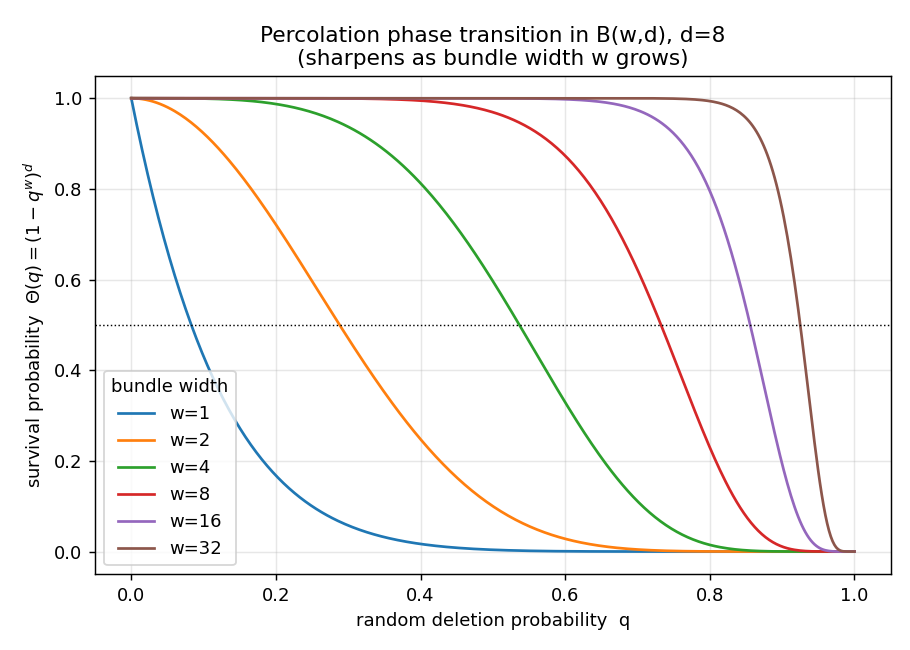
\includegraphics[width=0.78\linewidth]{figures/fig1_phase_transition.png}
\caption{Random survival probability $\Theta(q)=(1-q^w)^d$ for fixed depth $d$ as the
redundancy width $w$ grows. The curve steepens toward a step at $q_c\to 1$
(Theorem~\ref{thm:c3}, parts 1--2): wider redundancy makes the behavior robust to
random damage up to an ever-higher deletion fraction.}
\label{fig:phase}
\end{figure}

\begin{figure}[ht]
\centering
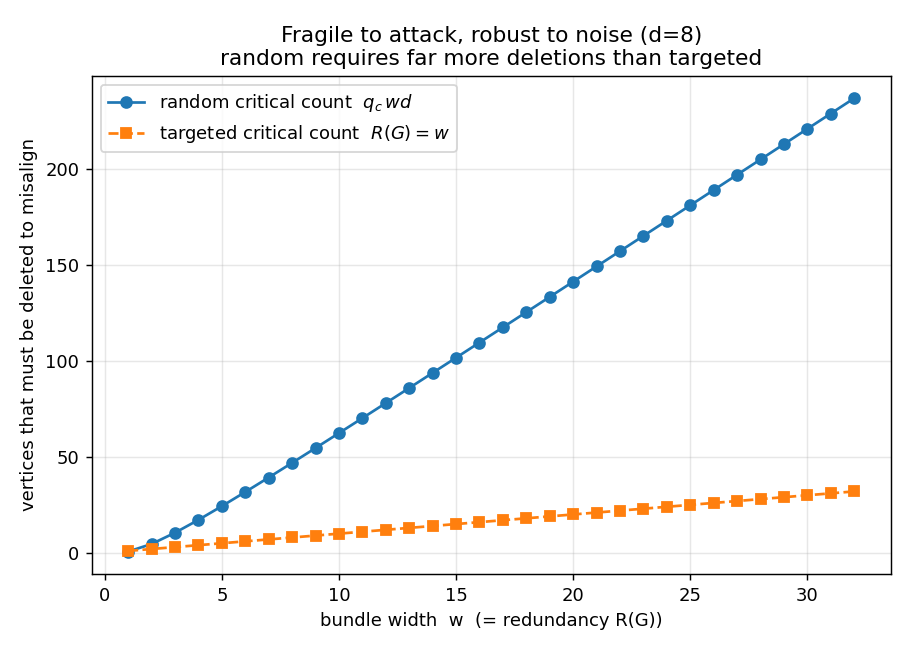
\includegraphics[width=0.78\linewidth]{figures/fig2_random_vs_targeted.png}
\caption{Critical ablation counts versus redundancy width $w$. The targeted attacker
removes only the $w$ vertices of the min-cut (Theorem~\ref{thm:c1}), whereas a random
adversary must delete $q_c\,wd$ vertices in expectation; the gap widens with $w$
(Theorem~\ref{thm:c3}, part 3).}
\label{fig:separation}
\end{figure}

\section{Discussion}
\label{sec:discussion}

\subsection{A unifying picture for contradictory reports}

The central contribution of the framework is conceptual: a single computation carries
two robustness numbers, the min-cut $R(G)$ that governs a targeted attacker and the
percolation threshold $q_c$ that governs random damage, and Theorem~\ref{thm:c3} shows
that these diverge as the redundancy width grows. The literature's contradictory
findings then become statements about different threat models applied to the same
circuit. Table~\ref{tab:reconcile} maps the principal empirical observations onto the
framework.

\begin{table}[ht]
\centering
\caption{The framework reads the field's contradictory findings as consistent
statements about distinct robustness numbers of the same circuit.}
\label{tab:reconcile}
\renewcommand{\arraystretch}{1.2}
\begin{tabular}{p{0.46\linewidth}p{0.46\linewidth}}
\toprule
\textbf{Empirical finding} & \textbf{Framework reading} \\
\midrule
Backup name-mover heads: ablating three heads drops the logit difference by
$5\%$ \cite{wang2022ioi} &
Large random robustness; surviving vertex-disjoint paths
(Theorems~\ref{thm:c1}--\ref{thm:c2}). \\
``Redundant paths survived ablation'' \cite{joad2026directions}; refusal cones of
dimension $\le 5$ \cite{wollschlager2025cones} &
$k$-redundancy with $R(G)>1$ (Theorems~\ref{thm:a2},~\ref{thm:c1}); latent and
pre-existing (Proposition~\ref{prop:d1}). \\
Self-repair restoring $\approx 70\%$ of the logit reduction \cite{mcgrath2023hydra} &
The surviving pathways already held the information
(Proposition~\ref{prop:d1}, Theorem~\ref{thm:a1}). \\
Safety removable in $\approx 5$ steps \cite{qi2023finetuning}; shallow and
first-token \cite{qi2024shallow} &
Small effective $R(G)$, hence a tiny targeted budget
(Corollary~\ref{cor:e1}). \\
A single refusal direction \cite{arditi2024refusal} &
The special case $R(G)=1$: the min-cut is the one direction
(Example~\ref{ex:shallow}). \\
\bottomrule
\end{tabular}
\end{table}

\subsection{Relation to the compensatory effect}

The logit-level compensatory effect of \cite{mcgrath2023hydra} is layer-granular and,
as \cite{rushing2024selfrepair} document, roughly $30\%$ of it is a LayerNorm-scaling
artifact rather than genuine rerouting. Theorem~\ref{thm:a1} replaces it with the exact
identity $\Delta I_i=\II(S;R_i\mid R_{-i})$, which by construction discards the
information $R_i$ shares with the other pathways and so carries no scaling artifact.
The result is a head- or feature-level, mechanism-corrected measure of how much a
pathway genuinely contributes that no other pathway can supply.

\subsection{The size of the effect}

The targeted-versus-random separation is not marginal. At depth $d=8$ and width
$w=16$, a random adversary must delete about $110$ of the $128$ internal units---$86\%$
of them---to match the damage a targeted adversary inflicts by removing the $16$
min-cut vertices, $12.5\%$ of the network (Table~\ref{tab:c3}). This is a roughly
sevenfold gap in raw count and a qualitative gap in fraction ($q_c=0.86$ against the
targeted $1/d=0.125$). Redundancy buys a great deal of robustness against
undirected damage and almost none against an adversary who attacks the cut.

\subsection{Limitations}

We state the framework's boundaries honestly.

\begin{itemize}[leftmargin=*,itemsep=2pt,topsep=2pt]
  \item \emph{Combinatorial idealization.} The graph model treats $S$ as computable
    only if a path is fully intact. Real transformers are analog: sub-threshold
    contributions along several partially damaged paths can sum past a decision
    threshold, so the min-cut $R(G)$ can \emph{under}-state true robustness. The exact
    survival law of Theorem~\ref{thm:c2} also assumes complete bipartite wiring between
    bundles; sparser wiring changes the constants but not the qualitative transition.
  \item \emph{Estimation on real models.} Computing $\Delta I_i=\II(S;R_i\mid R_{-i})$
    requires estimating conditional mutual information in high dimensions, which is
    hard and biased; the partial-information cross-check used here can over-report
    redundancy. We did not instantiate the bounds on an actual LLM---this is a theory
    plus synthetic-verification contribution, not an empirical measurement.
  \item \emph{Fano gives a floor.} Theorem~\ref{thm:b1} lower-bounds the behavioral
    error; it does not assert that the floor is achieved (it is tight when $S\mid
    R_{T^c}$ is uniform on its support).
  \item \emph{Static $R(G)$.} Corollary~\ref{cor:e1} bounds the budget to misalign at
    a fixed network but does not model how $R(G)$ itself evolves under training.
  \item \emph{Mapping behavior to a variable.} Real aligned behavior is not a single
    discrete variable; the framework applies per chosen behavior $S$.
\end{itemize}

\subsection{Open questions}

\begin{itemize}[leftmargin=*,itemsep=2pt,topsep=2pt]
  \item \emph{Dynamics of $R(G)$ under training.} Determine conditions under which
    adversarial or continued training grows the alignment min-cut rather than cutting
    it. The capacity bound of \cite{hanni2024superposition} and the
    abundance/scarcity regimes of \cite{bereska2025superposition} are candidate
    predictors.
  \item \emph{Analog-threshold percolation.} Replace ``path intact'' by ``summed
    contribution exceeds a threshold $\theta$'' and derive the corresponding weighted
    min-cut and flow threshold, lifting the combinatorial idealization.
  \item \emph{Degeneracy beyond the single min-cut.} Port the networked-buffering and
    degeneracy notions of \cite{whitacre2010degeneracy} to bound multi-pathway lesion
    robustness by a graph quantity richer than the single min-cut.
  \item \emph{Tight behavioral bounds.} Develop list-decoding analogues of
    Theorem~\ref{thm:b1} for graded refusal behaviors and relate the decoder error
    $P_e$ quantitatively to the output robustness $\rho$ for vector behaviors.
  \item \emph{Estimator-robust ablation.} Design a redundancy-aware estimator of
    $\Delta I_i$ that resists the underestimation of single-head ablation reported at
    scale by \cite{frank2026routing}.
\end{itemize}

\section{Conclusion}
\label{sec:conclusion}

We have given a self-contained mathematical framework for the compensatory robustness
of aligned behavior in language models, and answered the motivating question
affirmatively but with a precise caveat. On the information side, the cost of ablating
a pathway is exactly its non-redundant conditional mutual information
$\II(S;R_i\mid R_{-i})$ (Theorem~\ref{thm:a1}), fully redundant pathways cost nothing,
$k$-redundancy buys resilience to any $k-1$ ablations (Theorem~\ref{thm:a2}), and Fano's
inequality turns this information loss into a provable floor on behavioral error
(Theorem~\ref{thm:b1}); when behavior survives, the surviving pathways must already have
carried the signal, so compensation reveals rather than creates redundancy
(Proposition~\ref{prop:d1}). On the graph side, the targeted critical threshold equals
the minimum vertex cut $R(G)$ (Theorem~\ref{thm:c1}), random survival obeys the exact
law $(1-q^w)^d$ (Theorem~\ref{thm:c2}), and the two thresholds are exponentially
separated by a percolation phase transition whose critical point tends to one and whose
width shrinks like $1/w$ (Theorem~\ref{thm:c3}).

The key takeaway is that a single aligned circuit can be robust to random damage and
fragile to a targeted attack at the same time, because these are governed by two
different invariants---the percolation threshold $q_c$ and the min-cut $R(G)$. This
dissolves the apparent contradiction between the field's fragile and distributed
reports, and shows that the premise of intrinsic robustness holds only in the
random/benign regime: a targeted adversary needs to degrade just $R(G)$ pathway-units
(Corollary~\ref{cor:e1}), which is cheap when alignment is shallow. Every nontrivial
claim was confirmed computationally---the ablation identity to machine precision, the
Fano floor without violation, the targeted threshold exactly equal to $R(G)$, and the
random survival law within Monte-Carlo confidence intervals.

Future work should lift the combinatorial idealization to analog-threshold
percolation, model how the alignment min-cut $R(G)$ evolves under adversarial and
continued training, and estimate the bounds on real transformers with redundancy-aware
estimators of conditional mutual information. Each of these would move the framework
from a synthetic-verification contribution toward a practical diagnostic of which kind
of robustness a deployed model's safety actually has.


\bibliographystyle{amsplain}
\bibliography{references}

\end{document}
